
\usetikzlibrary{calc}
\usetikzlibrary{chains, decorations.pathreplacing, positioning}


\definecolor{decoration}{RGB}{0, 122, 195} %CTU blue
\definecolor{heading}{RGB}{0, 122, 195}
\definecolor{headbackgroundgray}{RGB}{199, 219, 241} %light blue
\definecolor{backgroundgray}{RGB}{199, 219, 241} %CTU light blue
\definecolor{headgray}{rgb}{0.50,0.50,0.51}
\definecolor{enumgray}{RGB}{0, 122, 195} %CTU blue

%

\tdplotsetmaincoords{80}{40}

\captionsetup{labelsep=space,indention=-2cm,labelfont=bf,width=.9\textwidth,skip=.5\baselineskip}
\captionsetup[sub]{labelfont=bf,labelsep=period,labelformat=simple}

\setlength{\extrarowheight}{1pt}

\newcolumntype{Y}{>{\centering\arraybackslash}X}
\newcolumntype{Z}{>{\centering\arraybackslash}l}

\begin{figure}[!hp]
  \floatsetup{font=normalsize, rowpostcode = largevskip}

  \floatbox{figure}
  { %
    \begin{subfloatrow}[2]

    \ffigbox[\FBwidth]{%
      \resizebox{0.5\textwidth}{!}{%
      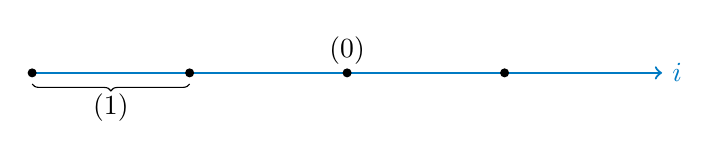
\begin{tikzpicture}[scale=2]%
        \tikzstyle{annot} = [text width=4em, text centered]
        \tikzstyle{axis} = [->, enumgray,thick]

        \draw[axis](0,0) -- (4,0) node[anchor=west] {$i$};

        \foreach \x in {0, ..., 3}{
          \node[draw,circle,inner sep=1pt,fill] (vertex\x) at (\x,0) {};
        }

        \node[annot, above of=vertex2, node distance=8pt] {(0)};
        \draw [decorate, decoration = {brace, mirror, raise = 4pt}] (0, 0) -- (1, 0) node[pos=0.5,below=4pt,black] {(1)};
      \end{tikzpicture}%
      }%

      \caption{One-dimensional grid}%
    }%

    \ffigbox[\FBwidth]{%
      \resizebox{0.5\textwidth}{!}{%
      \begin{tikzpicture}[scale=1.5]%
        \tikzstyle{annot} = [text width=4em, text centered];
        \tikzstyle{axis} = [->, enumgray,thick];
        \tikzstyle{edge} = [thick,black];
        \tikzstyle{selectedEdge} = [thick,enumgray];
        \tikzstyle{dashEdge} = [style=help lines,dashed];
        \tikzstyle{vertex} = [draw,circle,inner sep=1pt,fill];

        \draw [->, thick,enumgray] (0,0) -- (0,4) node[anchor=east] {$j$};
        \draw [->, thick,enumgray] (0,0) -- (6,0) node[anchor=west] {$i$};

        \foreach \x in {0, ..., 5}{
          \foreach \y in {0, ..., 3} {
            \ifthenelse { \not {\x = 5} \AND \not{\y = 0} }
              {
                \draw [edge] (\x,\y) -- (\x+1,\y);
              }{}

            \ifthenelse { \not {\y = 3} \AND \not{\x = 0} }
              {
                \draw [edge] (\x,\y) -- (\x,\y+1);

              }{}

            \ifthenelse { \x = 5 }{
              \draw [dashEdge] (\x,\y) -- (\x+1,\y);
            }{}

            \ifthenelse { \y= 3 }{
              \draw [dashEdge] (\x,\y) -- (\x,\y+1);
            }{}

            \ifthenelse { \y = 2 \AND \x = 2 }{
              \node[vertex,enumgray] (vertex\x\y) at (\x,\y) {};
            }{
              \node[vertex] (vertex\x\y) at (\x,\y) {};
            }
          }
        }

        \node[annot, above right of=vertex22, node distance=12pt] {(2)};

        \draw [decorate, decoration = {brace, mirror, raise = 4pt}] (3.04, 1) -- (3.96, 1) node[pos=0.5,below=4pt,black] {(3)};
        \draw [decorate, decoration = {brace, raise = 4pt}] (1, 1.04) -- (1, 1.96) node[pos=0.5,left=4pt,black] {(4)};

        \draw[fill=enumgray, fill opacity=0.3] (4,2) rectangle (5,3);
        \node[label] at (4.5,2.5) {(5)};
      \end{tikzpicture}%
      }%

      \caption{Two-dimensional grid}%
    }%

    \end{subfloatrow}%

    %

    \begin{subfloatrow}[1]
    \ffigbox[\FBwidth]{%
      \resizebox{0.45\textwidth}{!}{%
      \begin{tikzpicture}[scale = 2, tdplot_main_coords]%
        \tikzstyle{annot} = [text width=4em, text centered];
        \tikzstyle{axis} = [->, enumgray,thick];
        \tikzstyle{edge} = [thick,black];
        \tikzstyle{selectedEdge} = [thick,enumgray];
        \tikzstyle{dashEdge} = [style=help lines,dashed];
        \tikzstyle{vertex} = [draw,circle,inner sep=1pt,fill];

        \draw [->, thick,enumgray] (0,0,0) -- (4,0,0) node[anchor=north east] {$i$};
        \draw [->, thick,enumgray] (0,0,0) -- (0,7,0) node[anchor=south east] {$j$};
        \draw [->, thick,enumgray] (0,0,0) -- (0,0,4) node[anchor=south east] {$k$};

        \foreach \x in {0, ..., 3}{
          \foreach \y in {0, ..., 3} {
            \foreach \z in {0, ..., 3} {
              \ifthenelse { \not {\x = 3} \OR \z = 0 }
              {
                \ifthenelse { \z = 3 \OR \( \y = 0 \AND \not {\z = 0} \) } {
                  \draw [edge] (\x,\y,\z) -- (\x+1,\y,\z);
                } {
                  \draw [dashEdge] (\x,\y,\z) -- (\x+1,\y,\z);
                }
              }{}

              \ifthenelse { \not {\y = 3} \OR \z = 0 }
              {
                \ifthenelse { \x = 3 \OR \( \z = 3 \AND \not {\y = 3} \) } {
                  \draw [edge] (\x,\y,\z) -- (\x,\y+1,\z);
                } {
                  \draw [dashEdge] (\x,\y,\z) -- (\x,\y+1,\z);
                }
              }{}

              \ifthenelse { \not {\z = 3} \OR \x = 0  }
              {
                \ifthenelse { \x = 3 \OR \( \y = 0 \AND \not { \x = 0} \) } {
                  \draw [edge] (\x,\y,\z) -- (\x,\y,\z+1);
                }{
                  \draw [dashEdge] (\x,\y,\z) -- (\x,\y,\z+1);
                }
              }{}

              \ifthenelse { \y = 1 \AND \x = 3 \AND \z = 1 }{
                \node[vertex,enumgray] (vertex\x\y\z) at (\x,\y,\z) {};
              }{
                \node[vertex] (vertex\x\y\z) at (\x,\y,\z) {};
              }
            }
          }
        }

        \node[annot, above right of=vertex311, node distance=12pt] {(6)};

        % Edges
        \draw [decorate, decoration = {brace, mirror, raise = 4pt}] (2.04, 0,0) -- (2.96, 0,0) node[pos=0.5,below=4pt,black] {(7)};
        \draw [decorate, decoration = {brace, mirror, raise = 4pt}] (3,1.04,3) -- (3,1.96,3) node[pos=0.5,below=4pt,black] {(8)};
        \draw [decorate, decoration = {brace, mirror, raise = 4pt}] (3,3,2.04) -- (3,3,2.96) node[pos=0.5,right=4pt,black] {(9)};

        % Front right
        \draw[fill=enumgray, fill opacity=0.3] (3,2,0) -- (3,3,0) -- (3,3,1) -- (3,2,1) -- cycle;
        \node[label] at (3,2.5,0.5) {(12)};

        % Top
        \draw[fill=enumgray, fill opacity=0.3] (0,1,3) -- (0,2,3) -- (1,2,3) -- (1,1,3) -- cycle;
        \node[label] at (0.5,1.5,3) {(10)};

        % Top
        \draw[fill=enumgray, fill opacity=0.3] (0,0,0) -- (0,0,1) -- (1,0,1) -- (1,0,0) -- cycle;
        \node[label] at (0.5,0,0.5) {(11)};

        % Cube
        \draw[fill=enumgray, fill opacity=0.3] (2,0,2) -- (2,0,3) -- (3,0,3) -- (3,0,2) -- cycle;
        \draw[fill=enumgray, fill opacity=0.3] (3,0,3) -- (2,0,3) -- (2,1,3) -- (3,1,3) -- cycle;
        \draw[fill=enumgray, fill opacity=0.3] (3,0,2) -- (3,1,2) -- (3,1,3) -- (3,0,3) -- cycle;
        \node[label] at (2.5, 0,2.5) {(13)};

      \end{tikzpicture}%
      }%
    }{ \caption{Three-dimensional grid} }%
    \end{subfloatrow}%

    %

    \ffigbox[\FBwidth]{%
    \begin{tabularx}{\textwidth}{Y|Y|Y|Y|Y|Y}%
      \textbf{ID} & \textbf{Grid Dim.} & \textbf{Ent Dim.} & \textbf{Coordinate} & \textbf{Orientation} & \textbf{Basis} \\
      \hline \hline
      0 & 1 & 0 & (2) & 0 & (1)\\ \hline
      1 & 1 & 1 & (0) & 0 & (0)\\ \hline
      2 & 2 & 0 & (2, 2) & 0 & (1, 1) \\\hline
      3 & 2 & 1 & (3, 1) & 0 & (0, 1)\\
      4 & 2 & 1 & (1, 1) & 1 & (1, 0)\\\hline
      5 & 2 & 2 & (4, 2) & 0 & (0, 0)\\ \hline
      6 & 3 & 0 & (3, 1, 1) & 0 & (1, 1, 1)\\ \hline
      7 & 3 & 1 & (2, 0, 0) & 0 & (0, 1, 1)\\
      8 & 3 & 1 & (3, 1, 3) & 1 & (1, 0, 1)\\
      9 & 3 & 1 & (3, 3, 2) & 2 & (1, 1, 0)\\\hline
      10 & 3 & 2 & (0, 1, 3) & 0 & (0, 0, 1)\\
      11 & 3 & 2 & (0, 0, 0) & 1 & (0, 1, 0)\\
      12 & 3 & 2 & (3, 2, 0) & 2 & (1, 0, 0)\\ \hline
      13 & 3 & 3 & (2, 0, 2) & 0 & (0, 0, 0)\\
    \end{tabularx}%
    }

    \caption{All grid entities types for one-, two- and three-dimensional grids}%
    \label{fig:grid-entities}
  }

\end{figure}